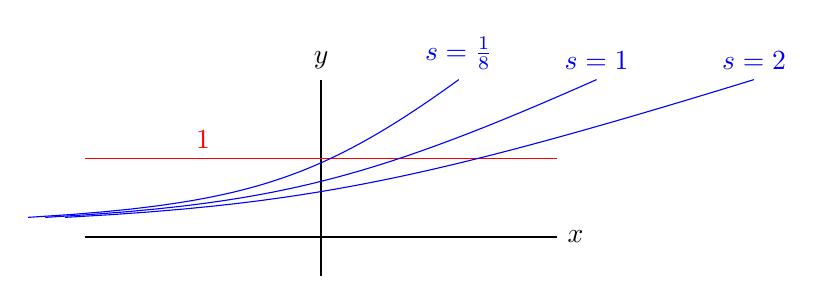
\begin{tikzpicture}
\draw[thick] (-3,0)--(3,0) node[right]{$x$};
\draw[thick] (0,-0.5)--(0,2) node[above]{$y$};

\draw[red] (-3,1) -- node[above, pos=0.25] {1} (3,1);

\draw[blue, domain=0.25:2, samples=50] plot({(1+1/8)*\x - 1/\x},{\x}) node[above] {$s=\frac{1}{8}$};
\draw[blue, domain=0.25:2, samples=50] plot({(1+1)*\x - 1/\x},{\x}) node[above] {$s=1$};
\draw[blue, domain=0.25:2, samples=50] plot({(1+2)*\x - 1/\x},{\x}) node[above] {$s=2$};

\end{tikzpicture}